\documentclass[handout]{beamer}
\usepackage[utf8]{inputenc}
\usepackage{graphics}
\mode<presentation> {
\usetheme{unc}}
\setbeamertemplate{navigation symbols}{} % To remove the navigation symbols from the bottom of all slides uncomment this line

\usepackage{graphicx} % Allows including images
\usepackage{booktabs} % Allows the use of \toprule, \midrule and \bottomrule in tables


\usepackage{hyperref}
\hypersetup{linkcolor=blue,colorlinks=true}


% Remove symbols
\beamertemplatenavigationsymbolsempty


%\usetheme{default}

\usefonttheme{serif}

%----------------------------------------------------------------------------------------
%	TITLE PAGE
%----------------------------------------------------------------------------------------


\title[International Finance]{\LARGE{International Finance: Portfolio Investment, Concessional Finance, and FDI}}
\author[POLI 150]{Steven Saroka}
\institute{POLI 150}
\date{26 March 2024 - 2 April 2024}


\begin{document}

\begin{frame}
\titlepage % Print the title page as the first slide
\end{frame}


%----------------------------------------------------------------------------------------
%	PRESENTATION SLIDES
%----------------------------------------------------------------------------------------

\begin{frame} 
	\frametitle{\LARGE{Announcements}}
	\begin{itemize}
		
		\item NO CLASS on Thursday 3/28 
		\\~\\ 
		\item PSSP module 2 open from 3/27 - 4/10 
		\\~\\
		
		
	\end{itemize}
\end{frame}

\begin{frame} 
	\frametitle{\LARGE{Class Overview}}
	\begin{itemize}
		
			\item Types of international financial relations 
			\\~\\ 
			\item International borrowing and foreign loans 
			\\~\\
			\item International financial institutions
			\\~\\
			\item Debtor-creditor strategic interactions
			\\~\\
			\item Concessional finance
			\\~\\
			\item FDI: Reasons, Types, and Conflicts 
	
	\end{itemize}
\end{frame}

\begin{frame} 
	\frametitle{\LARGE{Key Terms}}
	\begin{itemize}
		\item Portfolio investment
		\item Interest rate
		\item Financial crisis
		\item Default
		\item Austerity
		\item IMF
		\item Conditionality
	\end{itemize}
\end{frame}

\begin{frame} 
	\frametitle{\LARGE{Key Terms Continued}}
	\begin{itemize}
		\item Concessional Finance
		\item FDI
		\item MNC
		\item Obsolescing Bargain
		\item Bilateral investment treaty
		\item Investor-state dispute settlement
	\end{itemize}
\end{frame}

\begin{frame} 
\frametitle{\LARGE{Central Questions}}
    \centering
    \Large{Why and how is money invested internationally? What tensions are caused by such investing?}
\end{frame}

\begin{frame} 
\frametitle{\LARGE{International Investment Flows}}
\begin{figure}[ht!]
\centering
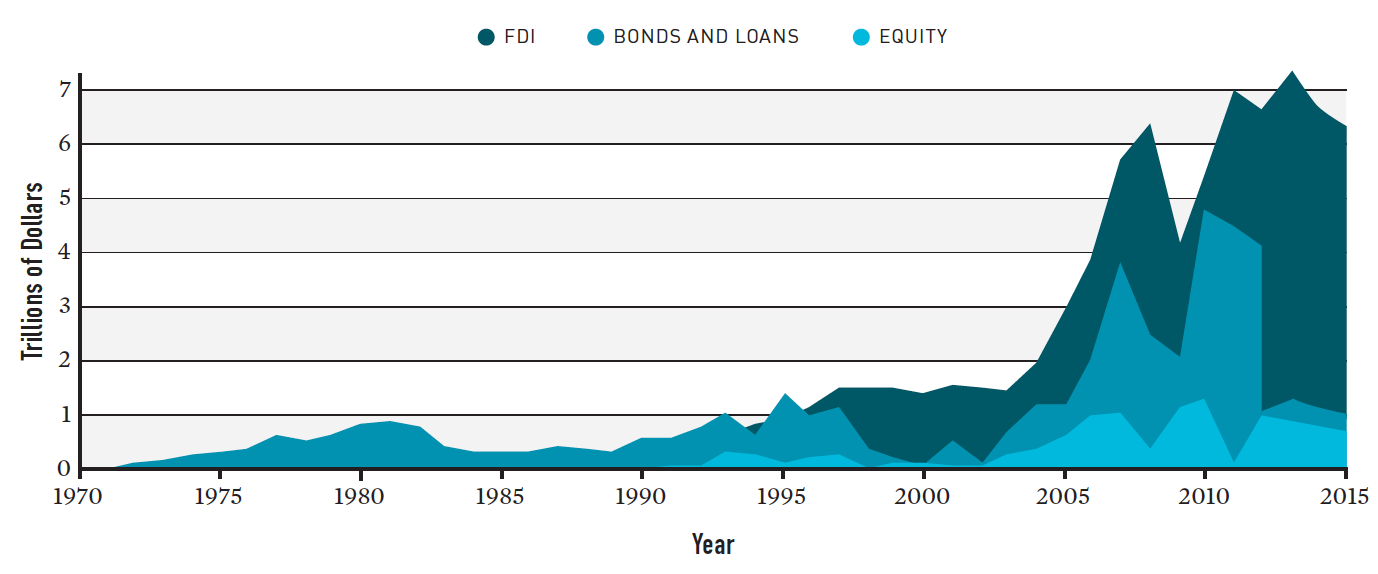
\includegraphics[width=\textwidth,height=0.8\textheight]{./invest.png}
\end{figure}
\end{frame}

\begin{frame} 
	\frametitle{\LARGE{Types of International Financial Flows}}
There are 3 types of international financial flows.
	\begin{enumerate}
		\item Portfolio Investment (slides 9-36)
		\item Concessional Finance (slides 38-40)
		\item Foreign Direct Investment	(slides 41-65)  
	\end{enumerate}

\end{frame}

\begin{frame} 
	\frametitle{\LARGE{Types of International Financial Flows}}
	\begin{itemize}
			\item \textbf{Portfolio investment}: purchase of financial products in a foreign country where investors do not have any managerial control over the businesses in which they are investing. This includes: \pause 
			\begin{itemize}
			    \item Bank loans \pause 
			    \item Stocks (equities) \pause
			    \item Derivatives and complex financial products \pause 
			    \item Bonds (including \textbf{sovereign lending} to governments)   
			 \end{itemize}
	\end{itemize}
\end{frame}

%from investopedia
\begin{frame} 
	\frametitle{\LARGE{Portfolio Investment Type Definitions}}
	\begin{itemize}
		\item \textbf{Bank loans}: agreement by a lender to loan a sum of money with a date of repayment and interest rate. \pause 
		\item \textbf{Stocks (equities)}: fractional shares of ownership of a company. \pause
		\item \textbf{Bonds}: like a loan, except tradeable on secondary markets. Issued by both corporations and states. The owner is a \textbf{creditor} of the entity that issued the bond (the \textbf{debtor}). \pause  
		\item \textbf{Derivatives} and complex financial products: see \href{https://www.investopedia.com/terms/d/derivative.asp}{here} for optional details. 
	 	\item \textbf{Sovereign Lending}: private-sector financial institutions in one state loan to the sovereign government of another state. 
	\end{itemize}
\end{frame}

%\begin{frame} 
%	\frametitle{\LARGE{Types of International Financial Flows}}
%	\begin{itemize}
%		\item \textbf{Foreign direct investment}: a multinational company investing in a foreign state by acquiring local facilities over which it has direct managerial control. \pause 
%		\item FDI, by definition, is done by \textbf{multinational corporations}: firms operating in at least 2 states, with production/service facilities outside their state of origin.
%		\item Concessional finance: loans with low/no interest to the poorest states, usually by international organizations (e.g. World Bank, AIIB) or rich states. \pause 
%		\begin{itemize}
%			\item Official development assistance (foreign aid) is also a form of this.
%		\end{itemize}
%	\end{itemize}
%\end{frame}

\begin{frame}{\LARGE Government Bonds}
    \centering
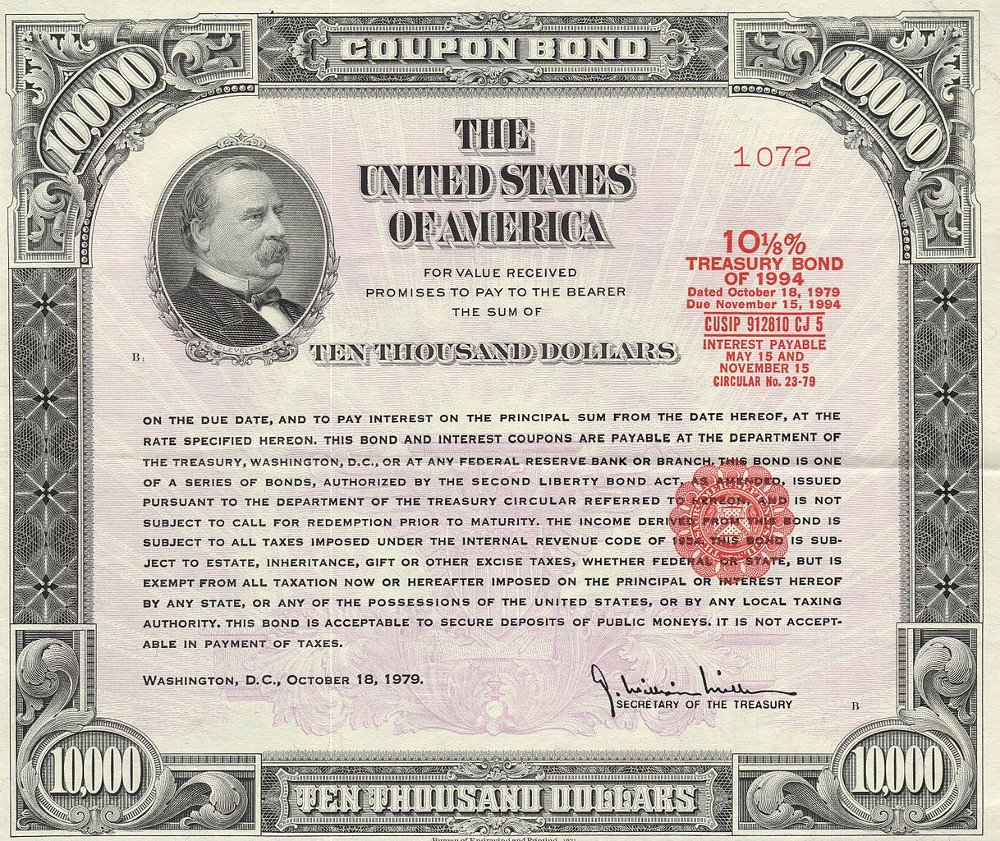
\includegraphics[width=\textwidth,height=0.8\textheight,keepaspectratio]{1979-10000-Treasury-Bond.jpg}
\end{frame}

\begin{frame}{\LARGE Eurozone Bond Rates}
	\centering
	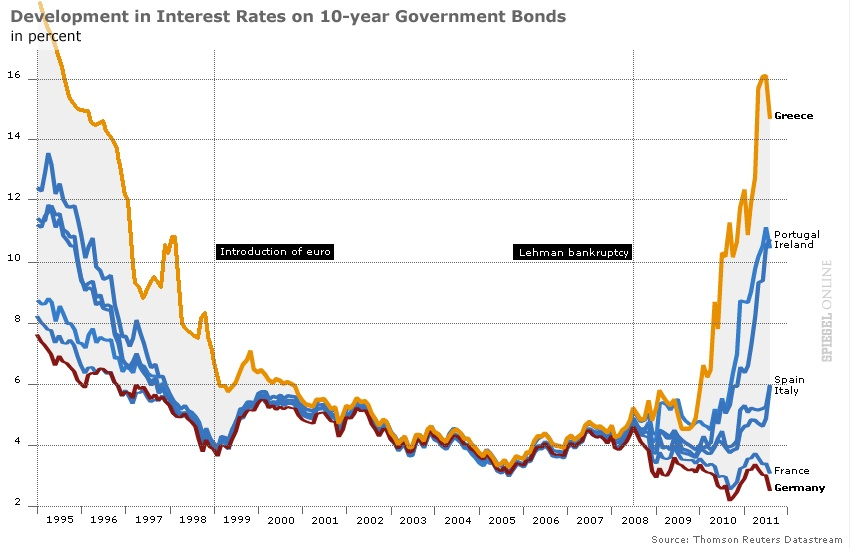
\includegraphics[width=\textwidth,height=0.8\textheight,keepaspectratio]{Eurozone rates.jpg}
\end{frame}



\begin{frame} 
	\frametitle{\LARGE{Why Does Money Move Internationally?}}
	\begin{itemize}

			\item \textbf{Money itself (capital) travels between states based on the interest rate of loans and bonds}, and the financial performance of stocks. \pause
			\item The return on loaning capital is driven by its interest rate. \pause
			\item In markets where capital is (relatively) scarce, that scarcity of supply increases the value of capital and thus increases the interest rates lenders can charge. \pause
			\item As developing states are by definition capital-scarce, we should see firms from capital-rich developed states investing their capital in developing states. \pause
			\item \textbf{But, a majority of capital flows occur between rich countries with lower interest rates. Why?}
		
	\end{itemize}
\end{frame}

\begin{frame} 
\frametitle{\LARGE{FDI by Area}}
\begin{figure}[ht!]
\centering
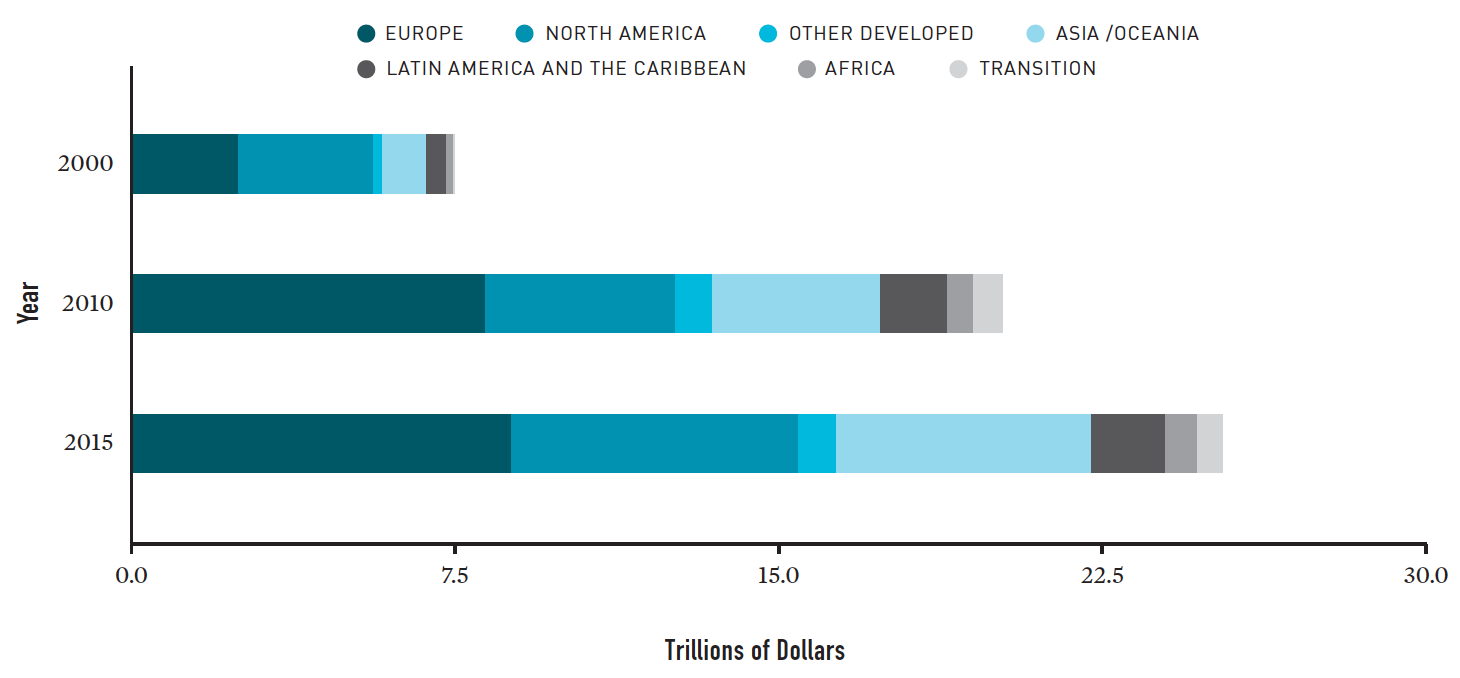
\includegraphics[width=\textwidth,height=0.8\textheight,keepaspectratio]{./fdiarea.png}
\end{figure}
\end{frame}

\begin{frame} 
	\frametitle{\LARGE{Why Does Money Move Internationally?}}
		\large{
			\begin{itemize}
			    \item The answer is found in the risk-return trade-off (political \textit{and} economic risk) of foreign investments. \pause 
			    \item The \textbf{incentive} for investing abroad is greater economic returns, in the form of higher interest rates and strong growth (for stocks, loans, bonds) and/or cheaper costs of production (for FDI). 
			    \item \textbf{The risk is that the foreign state make policy choices that devalue the investment.}
			\end{itemize}
		}
\end{frame}


\begin{frame} 
	\frametitle{\LARGE{Political Risks of Foreign Investment}}
	What kinds of political risks?
	\begin{itemize}
		\item Foreign governments can make policy choices that make investments less profitable, such as changing tax rates. \pause 
		\item In cases of FDI, the state may nationalize corporate property, creating losses for the corporation. \pause
		\item Political instability or war can also devalue investments and destroy property.
		\item Portfolio investment is volatile and prone to reversals. \pause 
		\item Crises and contagion are common, followed by austerity. \pause 
	\end{itemize}
	\textbf{All of this explains why a majority of capital investments are between already-developed rich countries, even though returns are lower.}
\end{frame}

\begin{frame} 
	\frametitle{\LARGE{Benefits of International Finance}}
However, international investment between developed and developing states does still occur. Why? There are still substantial benefits: \pause
	\begin{itemize}
			    \item Fund private and public sector activities \pause 
			    \item Promote economic growth \pause 
			    \item Transfer technologies and expertise (esp. FDI)  \pause
			    \item Higher returns than in ``safer" markets.		
	\end{itemize}
\end{frame}

\begin{frame} 
	\frametitle{\LARGE{Domestic Governance of Finance}}
	\begin{itemize}
			\item \textbf{Financial crises} are what happens when something goes wrong with this process of international investment. \pause
			\item The most common type of crisis associated with international finance is a \textbf{default}: failure by an actor to make payments on their debt. \pause
			\item When a corporation defaults, it generally goes bankrupt, with its remaining assets purchased by other firms. But this is not an option for a state.
			\item Financial/debt crises are common across time and space.
	\end{itemize}
\end{frame}

% Default waves picture 
\begin{frame}{\LARGE Waves of Default}
    \centering
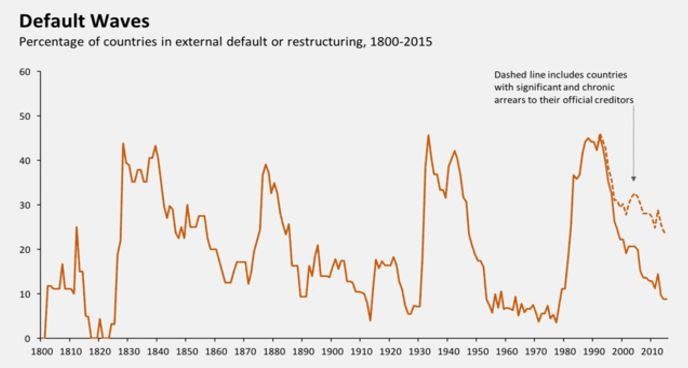
\includegraphics[width=\textwidth,height=0.8\textheight,keepaspectratio]{default waves.JPG}
\end{frame}

\begin{frame} 
	\frametitle{\LARGE{Anatomy of a Financial Crisis}}
	\begin{itemize}
		\item A state, or a significant sector of that state's economy, takes out loans from foreign actors. \pause
		\item Something threatens the ability of the debtor state/corporations to repay those loans. \pause
		\begin{itemize}
			\item Economic downturn that decreases demand for goods and services that provided revenues to make payments on those debts. \pause
			\item State instability or drastic shift in monetary policy (ex: election of a candidate promising to nationalize sectors of the economy). \pause
			\item Currency crisis (covered later).
		\end{itemize}
	\item Creditors begin to worry that they will not recoup their investment.
	\end{itemize}
\end{frame}

\begin{frame} 
	\frametitle{\LARGE{Anatomy of a Financial Crisis}}
	\begin{itemize}
		\item Creditors cease to approve new loans, and may (depending on the terms of the debt) call for immediate repayment in an attempt to secure their capital. \pause
		\item If one creditor does this, it is manageable. But if every creditor does this... \pause
		\item The debtor state, facing a sudden loss of financing and lacking a meaningful financial backstop, reduces or stops payment on its debts to avoid insolvency. \pause
		\item Current creditors entirely cease any remaining lending, while other potential sources of capital avoid this market due to the perceived risk of non-repayment. 	
	\end{itemize}
\end{frame}

\begin{frame} 
	\frametitle{\LARGE{Anatomy of a Financial Crisis}}
	\begin{itemize}
		\item The debtor state eventually runs out of reserves, cannot get new ones via lending as it normally would, and defaults. \pause
		\item If there are other debtor countries with similar economies, investor fear can spread, leading to a repeat of this cycle in other states. This is \textbf{financial contagion}. \pause
		\begin{itemize}
			\item This can spread the crisis even to states that were otherwise economically healthy - a self-fulfilling prophecy. \pause
		\end{itemize}
		\item At some point, debt restructuring negotiations begin.		
	\end{itemize}
\end{frame}

\begin{frame} 
	\frametitle{\LARGE{Domestic Governance of Finance}}
	\begin{itemize}
		\item How do governments respond to a financial crisis? Ideally, they  have a bundle of options... \pause
		\begin{itemize}
			\item Fiscal policy: bailouts from a Lender of Last Resort \pause 
			\item Monetary policy: reduce interest rates \pause 
			\item Regulation: prevent future vulnerabilities \pause
		\end{itemize}		
		\item But all of these have domestic and international costs, and are often influenced by creditor states during debt restructuring negotiations. 		
	\end{itemize}
\end{frame}

\begin{frame} 
	\frametitle{\LARGE{Crisis and Strategic Interactions}}
	\begin{itemize}
		\item A common response to repayment issues is \textbf{austerity}: application of policies to reduce state spending, usually involving cutting government programs, raising taxes, and cutting wages. \pause
		\item These measures have far-reaching negative consequences for citizens who had nothing to do with the financial crisis, creating a \textbf{bargaining interaction} over the scale of austerity measures between those citizens who will be hurt by them versus the state and affected economic sectors.
	\end{itemize}
\end{frame}

\begin{frame} 
	\frametitle{\LARGE{Crisis and Strategic Interactions}}
	\begin{itemize}
		\item Additionally, interactions between debtor and creditor states are also strategic. \pause
		\item A state in default (a debtor state) would prefer to have its debt entirely forgiven, while creditor states (those that loaned to it, either directly or via corporations headquartered in those states) want full repayment of their loans. \pause
		\item Debtors can threaten full default, while creditors can threaten to cut off future lending and freeze funds. \pause
		\item Additionally, there is a risk that investor panic may cause a crisis to spread from one state's markets to other similar states.
	\end{itemize}
\end{frame}

\begin{frame} 
	\frametitle{\LARGE{Crisis and Strategic Interactions}}
	\begin{itemize}
		\item Such an economic conflict is destructive, so both sides also have an incentive to negotiate. This resembles a bargaining problem with incomplete information about resolve.
		\item When such crises are resolved successfully, the debt is \textbf{restructured} so that (mostly) normal financial life can resume, but this may involve unpopular cutbacks and lingering austerity measures...
	\end{itemize}
\end{frame}

\begin{frame} 
	\frametitle{\LARGE{Governing International Finance}}
	\begin{itemize}
			\item Given the costs of financial crises and defaults, it is clear that financial stability is a public good. \pause 
			\begin{itemize}
			    \item Like all public goods in IR, it is undersupplied \pause 
                \item Governments, banks, firms need access to loans \pause 
                \item National governments do not serve as Lender of Last Resort (LLR) internationally \pause 
                \item Incentives to defect by under-regulating domestically and by self-interested macroeconomic policies  
			\end{itemize}
	\end{itemize}
\end{frame}

\begin{frame} 
	\frametitle{\LARGE{Governing International Finance}}
	\begin{itemize}
		\item International institutions step in to fill some of those roles: \pause 
		\begin{itemize}
			\item \textbf{International Monetary Fund (IMF)}: focuses on financial stability, serves as primary Lender of Last Resort. \pause 
			\item Bank for International Settlements: provides regulations for international, large banks. \pause 
			\item G-20: group of mostly rich developed states that coordinate macroeconomic policies, especially after the 2008 Financial Crisis.
		\end{itemize}
	\end{itemize}
\end{frame}

\begin{frame} 
	\frametitle{\LARGE{The International Monetary Fund}}
	\begin{itemize}
		\item The IMF was originally founded to manage the gold standard under the Bretton Woods monetary system.
		\item After the end of the gold standard in the 1970s, it adapted to stay relevant.
  		\item 1980s and after: its primary role is preventing the spread of economic and financial crises, and helping to contain them if they do spread.
  		\item Primary way it does this is by serving as the global \textbf{Lender of Last Resort}: a source of emergency loans to states in crisis that conventional capital sources deem too risky to invest in. 
	\end{itemize}
\end{frame}

\begin{frame} 
	\frametitle{\LARGE{The International Monetary Fund}}
	\begin{itemize}
		\item The IMF's financial resources come from contributions from its member governments. \pause 
		\begin{itemize}
			\item Larger contributions lead to greater voting power \pause 
			\item U.S. has largest share (18\%) followed by the EU (32\%) \pause 
			\item IMF rules require 85\% supermajority to take action.
		\end{itemize}
		\item IMF lending comes with conditions, often called \textbf{structural adjustment programs/conditionality}: \pause 
		\begin{itemize}
			\item These are conditions partially for economic growth, partially for IMF to manage its own lending risk. \pause 
			\item Requires a country to make economic reforms, usually cutting domestic spending via austerity measures. \pause 
			\item These reforms are controversial domestically. 
		\end{itemize}
	\end{itemize}
\end{frame}

%% IMF protests 
\begin{frame}{\LARGE Protesting IMF Programs}
    \centering
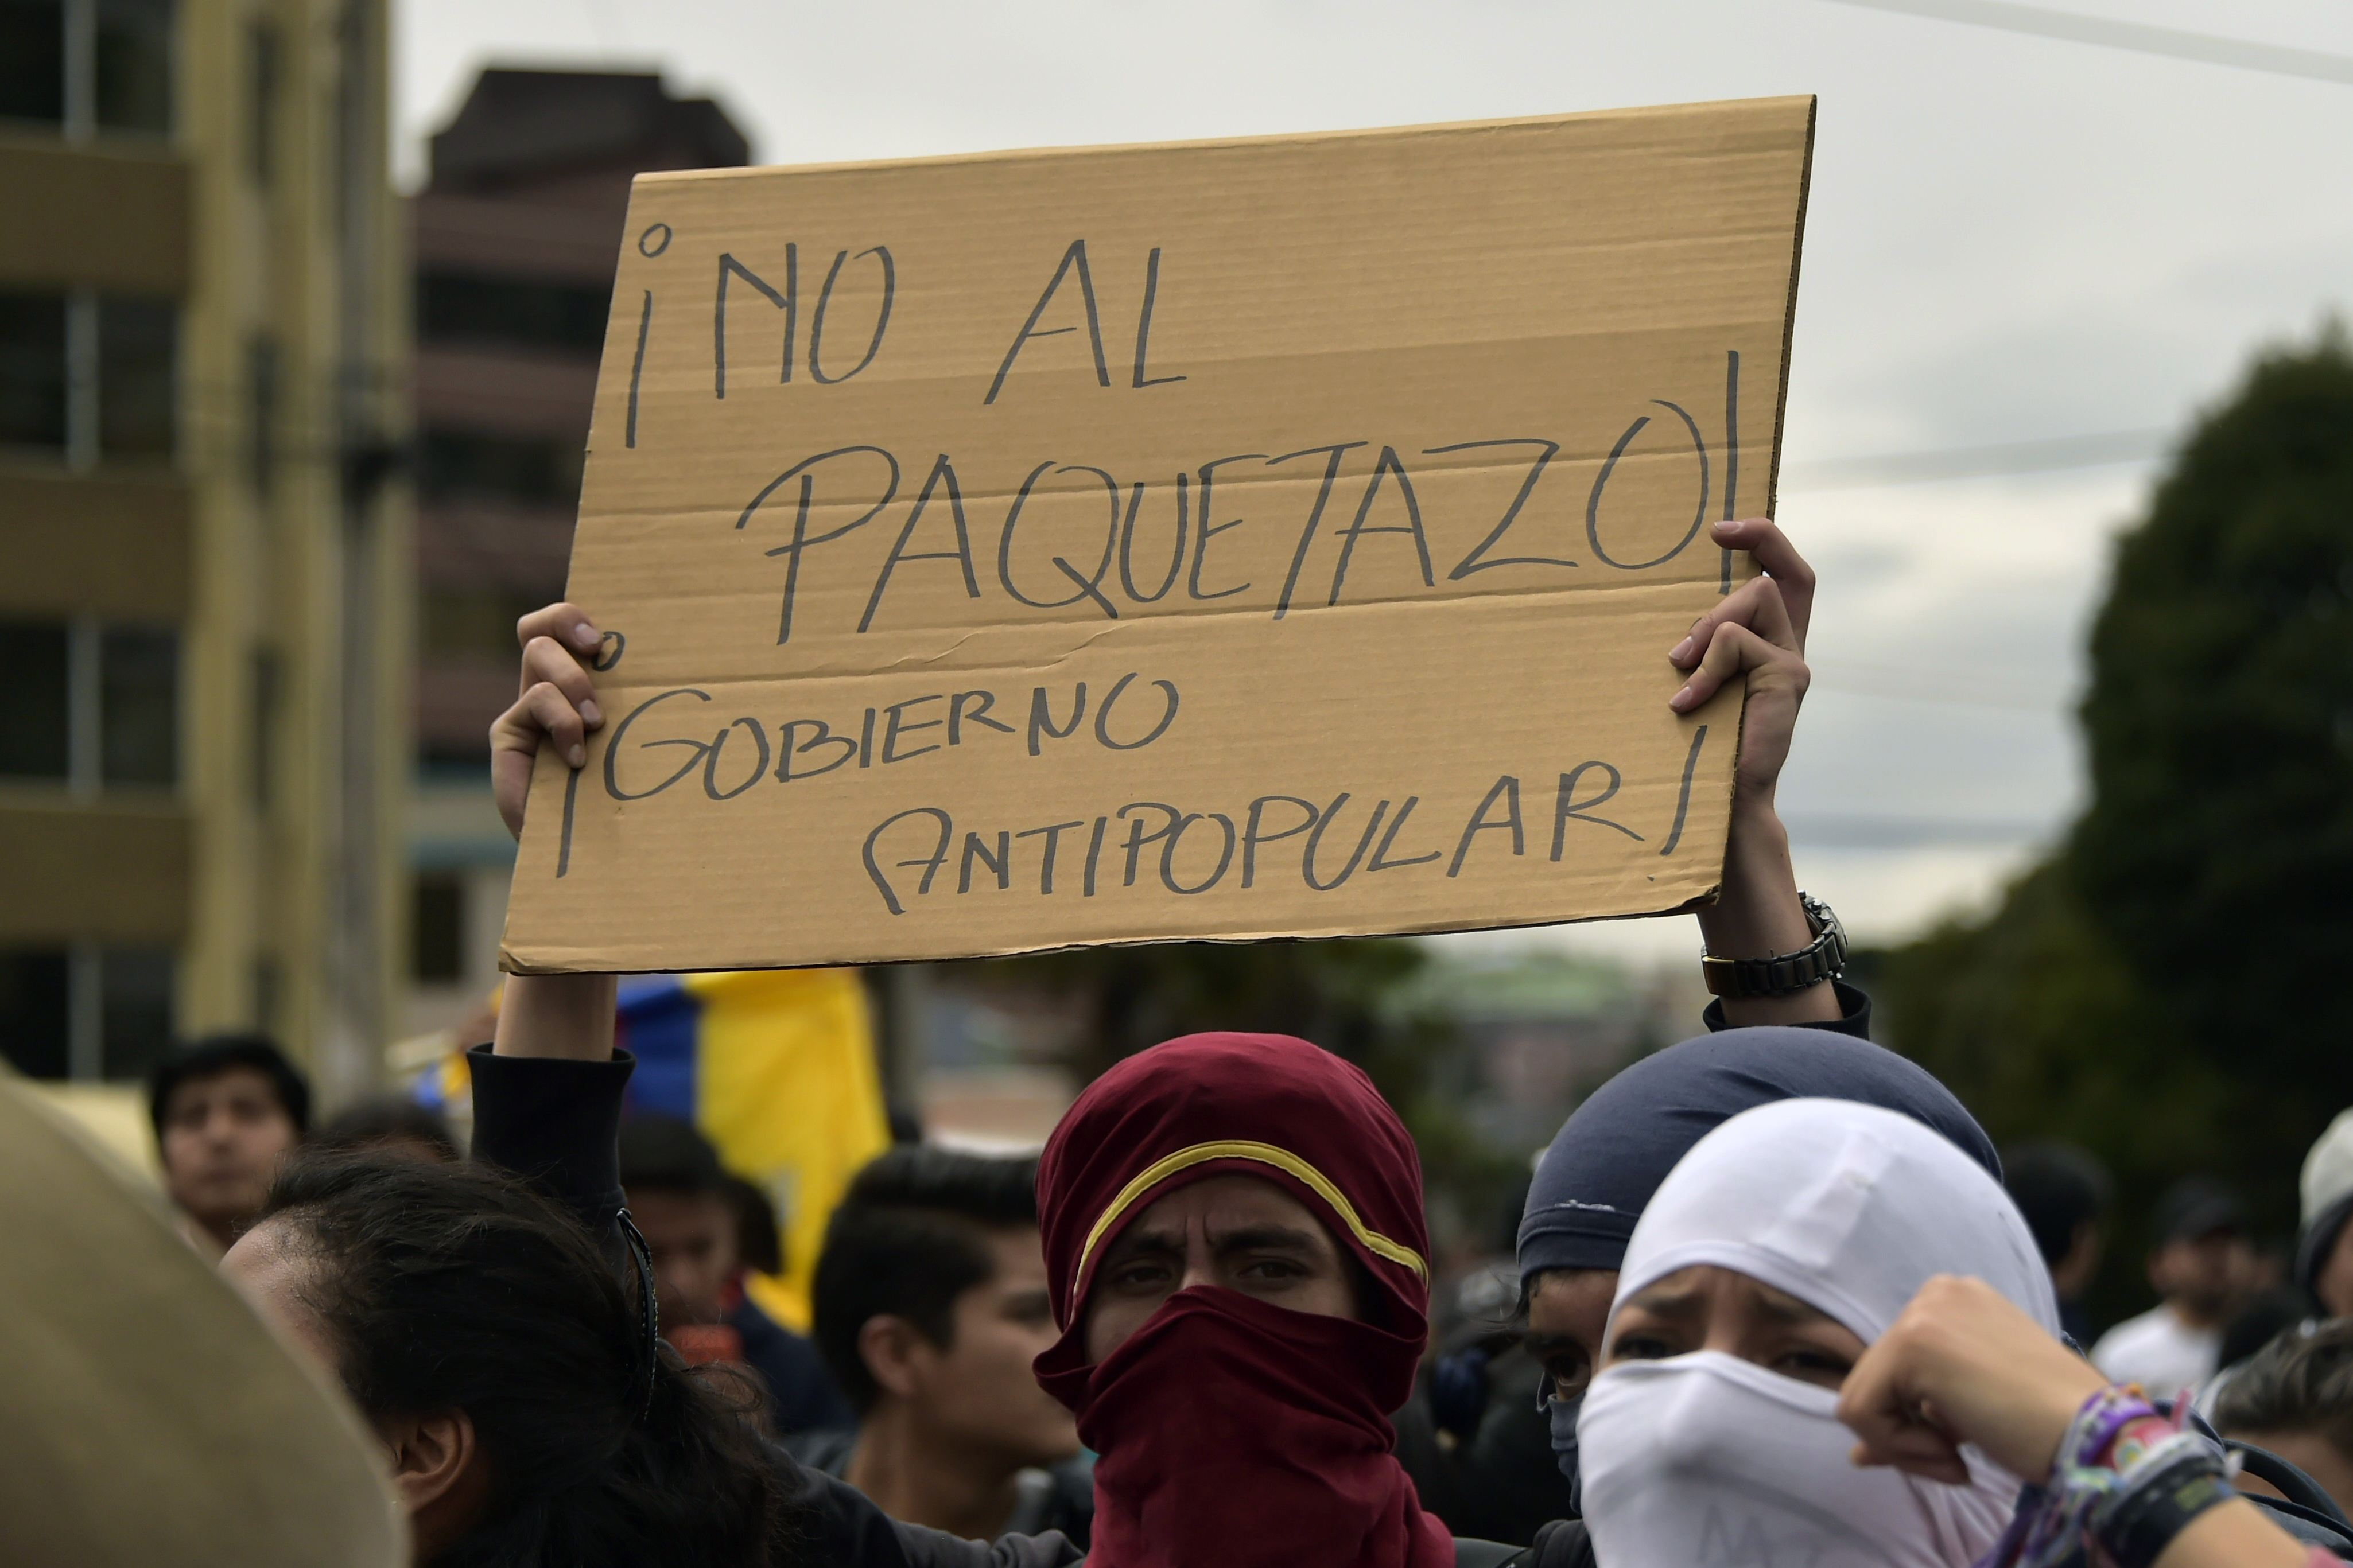
\includegraphics[width=\textwidth,height=0.8\textheight,keepaspectratio]{ecuador imf.jpg}
\end{frame}

\begin{frame} 
	\frametitle{\LARGE{Critiques of the IMF}}
	\begin{itemize}
		\large{
			\item Effects of liberalization on economic growth (especially structural adjustments) \pause 

			\item Effects of IMF lending on growth (do countries actually recover?) \pause 

			\item Conditions are not always enforced \pause 

			\item Moral hazard, as with any Lender of Last Resort \pause  

			\item Potentially a tool for international investors \pause 

			\item Bias due to domination by rich developed Western states.
		}
	\end{itemize}
\end{frame}

%\begin{frame} 
%	\frametitle{\LARGE{de Jonge 2017 Review}}
%Group yourselves and answer the following:
%	\begin{itemize}
%		\item What was de Jonge's main point?
%		\item How is the AIIB different from similar institutions like the IMF?
%	\end{itemize}
%\end{frame}

\begin{frame} 
	\frametitle{\LARGE{Alternative Institutions? The AIIB}}
	\begin{itemize}
			\item Asian Infrastructure Investment Bank (AIIB) is a very new (2015) international financial institution. \pause 
			\begin{itemize}
			    \item China's power in it is similar to the US' in the IMF. \pause 
			    \item China uses its trade income to generate investment returns, some of which help fund this. \pause
			 \end{itemize}
			\item As its name suggests, the AIIB loans to Asian countries (and some African states) to develop infrastructure. \pause 
			\begin{itemize}
			    \item Has also made several loans related to coronavirus response. \pause 
			    \end{itemize}
			\item The way the AIIB manages risk is quite different than the IMF. \pause 
			\begin{itemize}
			    \item Does not include the same structural adjustment reforms. \pause 
			    \item However, can include conditions of infrastructure ownership. \pause 
			    \item AIIB may not focus on traditional conditionality, but includes other conditions that benefit China.
		    \end{itemize}
	\end{itemize}
\end{frame}

\begin{frame} 
	\frametitle{\LARGE{Alternative Institutions? The AIIB}}
Implications of the AIIB:
	\begin{itemize}
		\item The AIIB means that the IMF is no longer the only entity that can act as a Lender of Last Resort. \pause
		\item Previously, states in financial crises that disliked IMF conditionality had no real other options. \pause
		\item AIIB provides an alternative to Western-dominated institutions, and may be less willing to cooperate with those institutions in traditional debt restructuring. \pause
	\end{itemize}
\end{frame}

% Capital controls economist picture
\begin{frame}{\LARGE Financial Liberalization Over Time}
    \centering
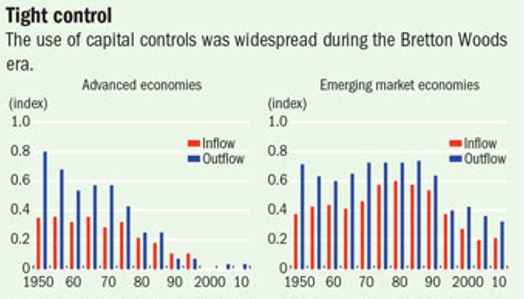
\includegraphics[width=\textwidth,height=0.8\textheight,keepaspectratio]{capital account.JPG}
\end{frame}

\begin{frame} 
	\frametitle{\LARGE{Why are International Flows Increasing?}}
In spite of financial crises, international capital flows have continued to increase in recent years. Why?
	\begin{itemize}
			\item Political reasons: response to crises. \pause 
			\begin{itemize}
			    \item Pressure from IMF and US \pause 
			    \item Some domestic groups benefit from liberalization and deregulation \pause
			    \item Potential for economic growth and interdependence \pause
			    \item Can be more beneficial to major powers, but still be Pareto-improving \pause 
			\end{itemize}
			\item Ideational: neoliberalism and the Washington Consensus \pause 
			\item Technological: more difficult to impose controls 
	\end{itemize}
\end{frame}

\begin{frame} 
	\frametitle{\LARGE{Types of International Financial Flows}}
	There are 3 types of international financial flows.
	\begin{enumerate}
		\item Portfolio Investment
		\item Concessional Finance
		\item Foreign Direct Investment
	\end{enumerate}
	Up to this point, we have discussed portfolio investment. The rest of these slides focus on \textbf{concessional finance} and then on \textbf{foreign direct investment}.
\end{frame}

\begin{frame} 
	\frametitle{\LARGE{Concessional Finance}}
	\begin{itemize}
		\item \textbf{Concessional finance}: giving or loaning money to the poorest developing states by both rich countries and intergovernmental organizations. \pause
		\item These states are generally considered too risky to invest in, necessitating a form of finance that is closer to aid than traditional investment. \pause
		\item The main international institution here is the \textbf{World Bank}. 	
	\end{itemize}
\end{frame}

\begin{frame} 
	\frametitle{\LARGE{Concessional Finance}: The World Bank}
	The \textbf{World Bank} is...
	\begin{itemize}
		\item Officially named the International Bank for Reconstruction and Development. \pause
		\item The third Bretton Woods institution, after the GATT/WTO and IMF, originally intended to promote economic development via loans following WWII. 
		\item After the end of the Bretton Woods monetary system in the 1970s, it shifted to generally providing affordable loans to developing states, usually for basic development projects. 
	\end{itemize}
\end{frame}

\begin{frame} 
	\frametitle{\LARGE{Concessional Finance}: The World Bank}
	\begin{itemize}
		\item The World Bank gets its funding by borrowing on member state financial markets, but usually at low rates due to its backing by member states. \pause
		\item The Bank is less prominent than IMF due to less conditionality around these loans, lack of private investor involvement, and smaller total amounts.
		\item It tends to deal in lower amounts than amounts of FDI, today's next topic...
	\end{itemize}
\end{frame}

\begin{frame} 
	\frametitle{\LARGE{FDI Central Questions}}
	\centering 
	\Large{Why do companies want to produce in other states? Why do those states let them in?}
\end{frame}

% FDI Overview
\begin{frame} 
	\frametitle{\LARGE{Foreign Direct Investment}}
	\begin{itemize}
		\item \textbf{Foreign direct investment}: a multinational company investing in a foreign state by acquiring local facilities over which it has direct managerial control. \pause 
		\item Another way to describe this is as the purchase of real assets that afford an MNC control over production.
		\item Multiple possible types of FDI: 
		\begin{itemize}
			\item Controlling stake in foreign entity \pause 
			\item Setting up new commercial operation \pause 
			\item Purchasing an existing commercial operation  
		\end{itemize}
		
	\end{itemize}
\end{frame}

% MNCs overview
\begin{frame} 
	\frametitle{\LARGE{Who Invests via FDI?}}
	\begin{itemize}
		\item \textbf{Multinational Corporations (MNCs):} firms operating in at least 2 states, with production/service facilities outside their state of origin. \pause 
		\item Any company doing FDI is by definition an MNC. \pause 
		\item MNCs can also sell and produce through sub-contracting, outsourcing, and globalized supply chains. 
	\end{itemize}
\end{frame}

% FDI inflows by region 
\begin{frame}{\LARGE FDI Inflows Regionally}
	\centering
	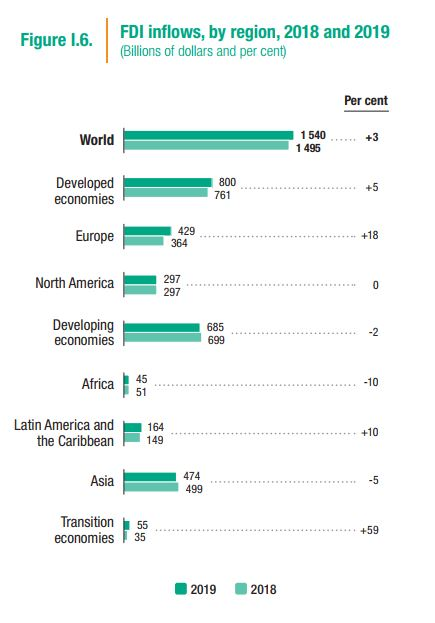
\includegraphics[width=\textwidth,height=0.9\textheight,keepaspectratio]{FDI inflows by region.JPG}
\end{frame}

\begin{frame} 
	\frametitle{\LARGE{Types of FDI}}
	Two kinds of FDI: horizontal and vertical.
	\begin{itemize}
		\item \textbf{Horizontal}: expanding a firm so that it is carrying out the same operations in \textit{home} and \textit{host} countries. \pause
		\item \textbf{Vertical}: a firm adding new business activities or breaking apart current ones into a chain spread across multiple states.
	\end{itemize}
\end{frame}


%% Coke - Horizontal FDI example
\begin{frame}{\LARGE Horizontal FDI: Coca-Cola}
	\centering
	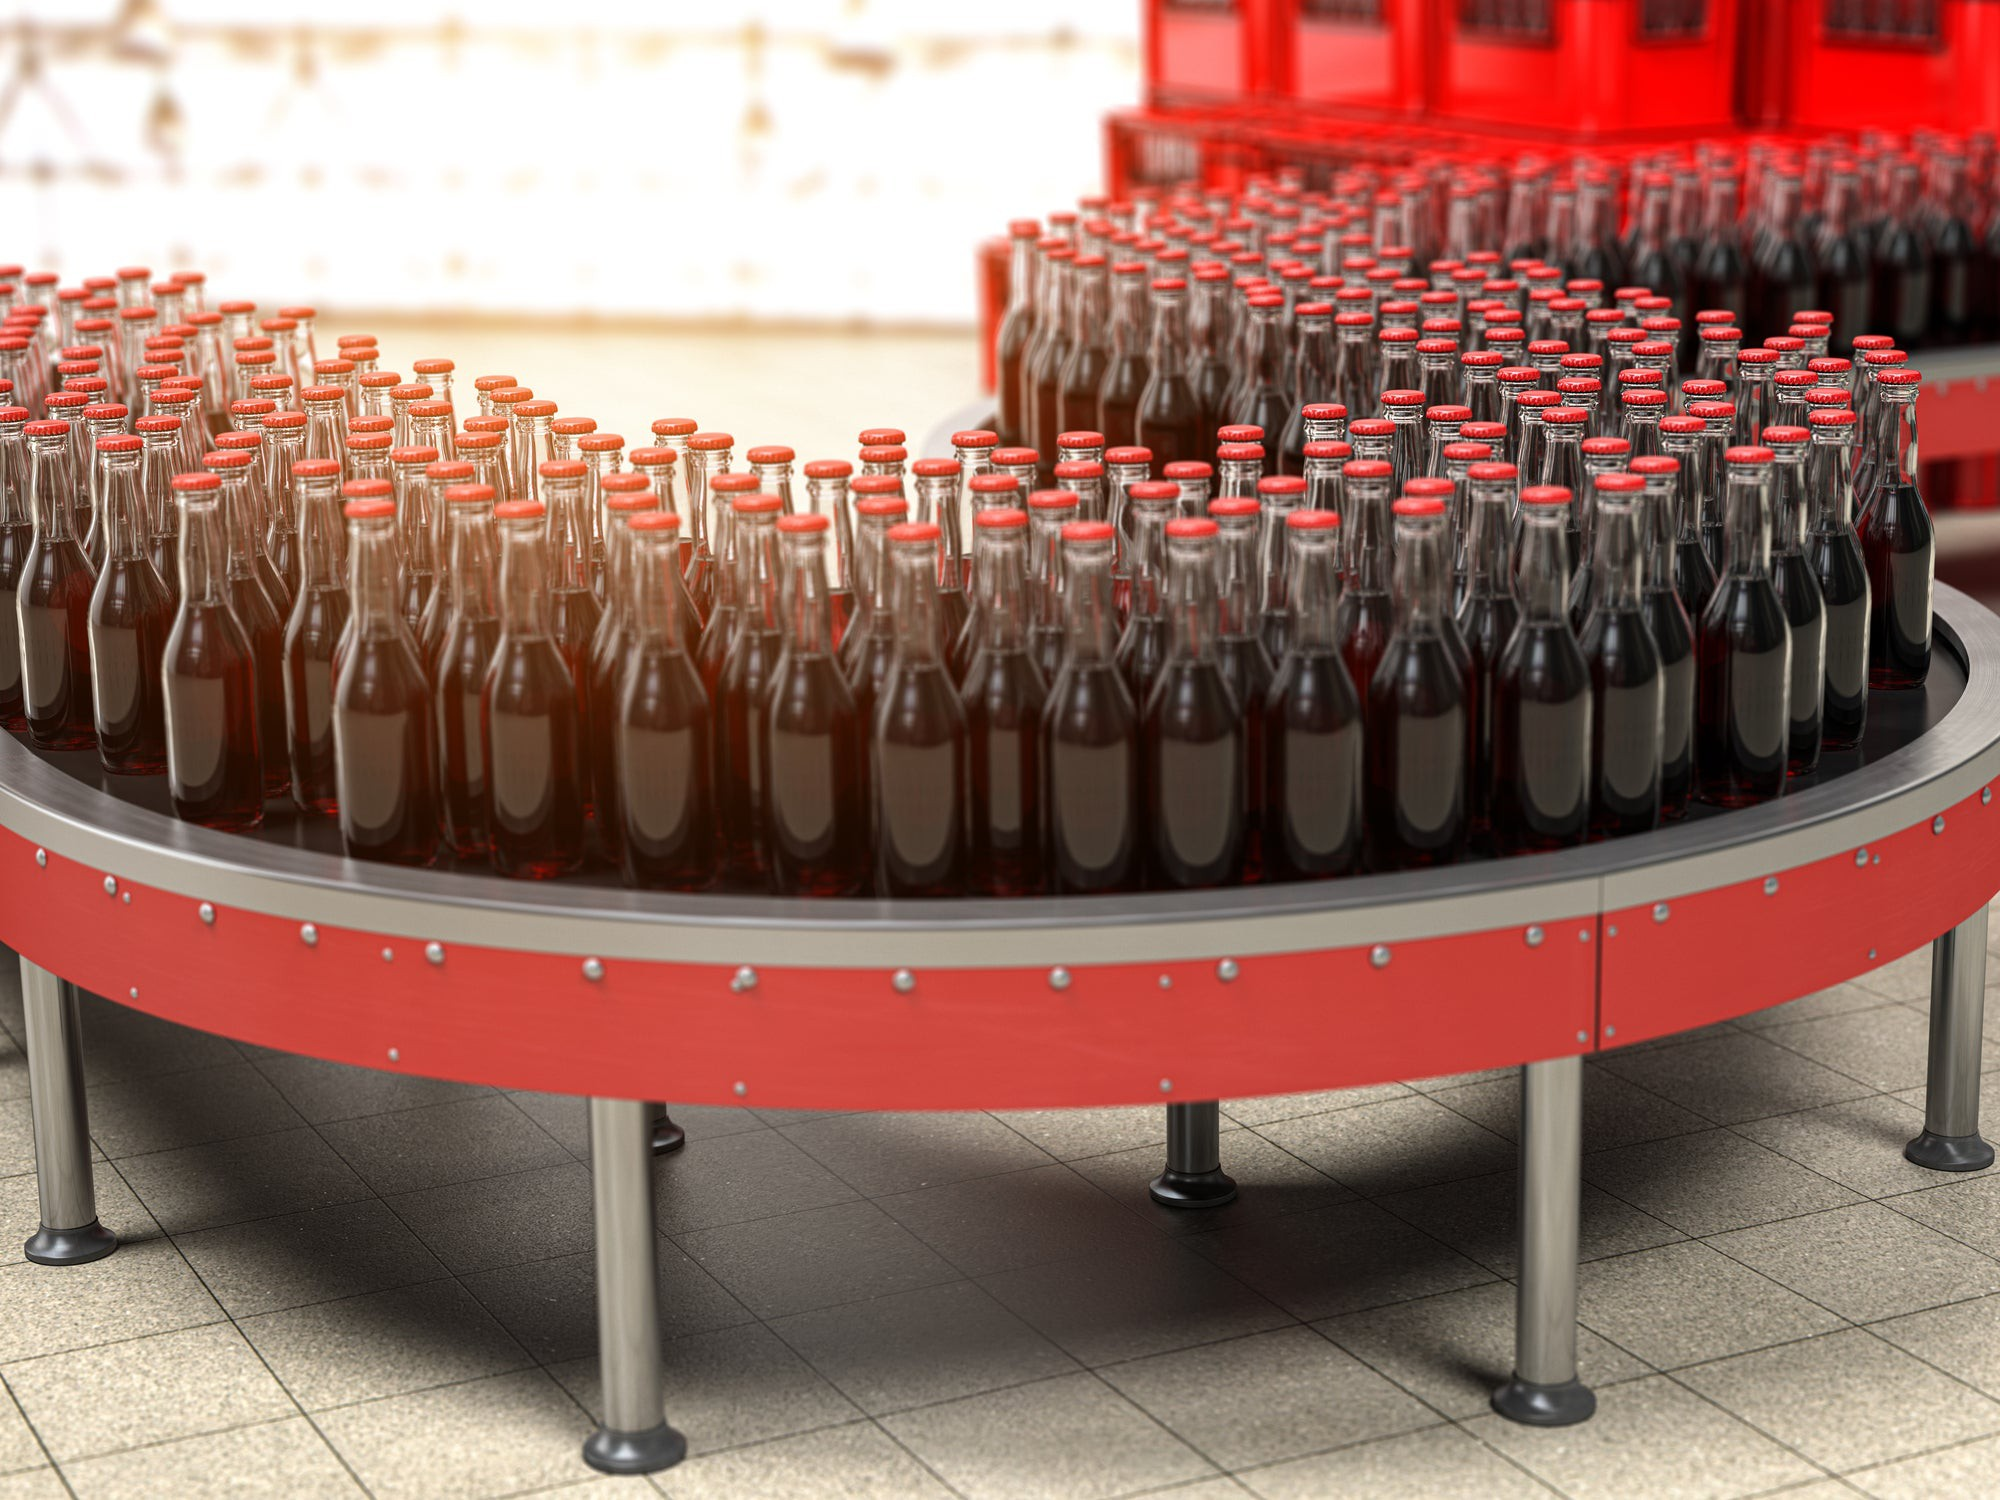
\includegraphics[width=\textwidth,height=0.8\textheight,keepaspectratio]{Coca Cola.jpg}
\end{frame}

%% Ford - Vertical FDI example 
\begin{frame}{\LARGE Vertical FDI: Ford}
	\centering
	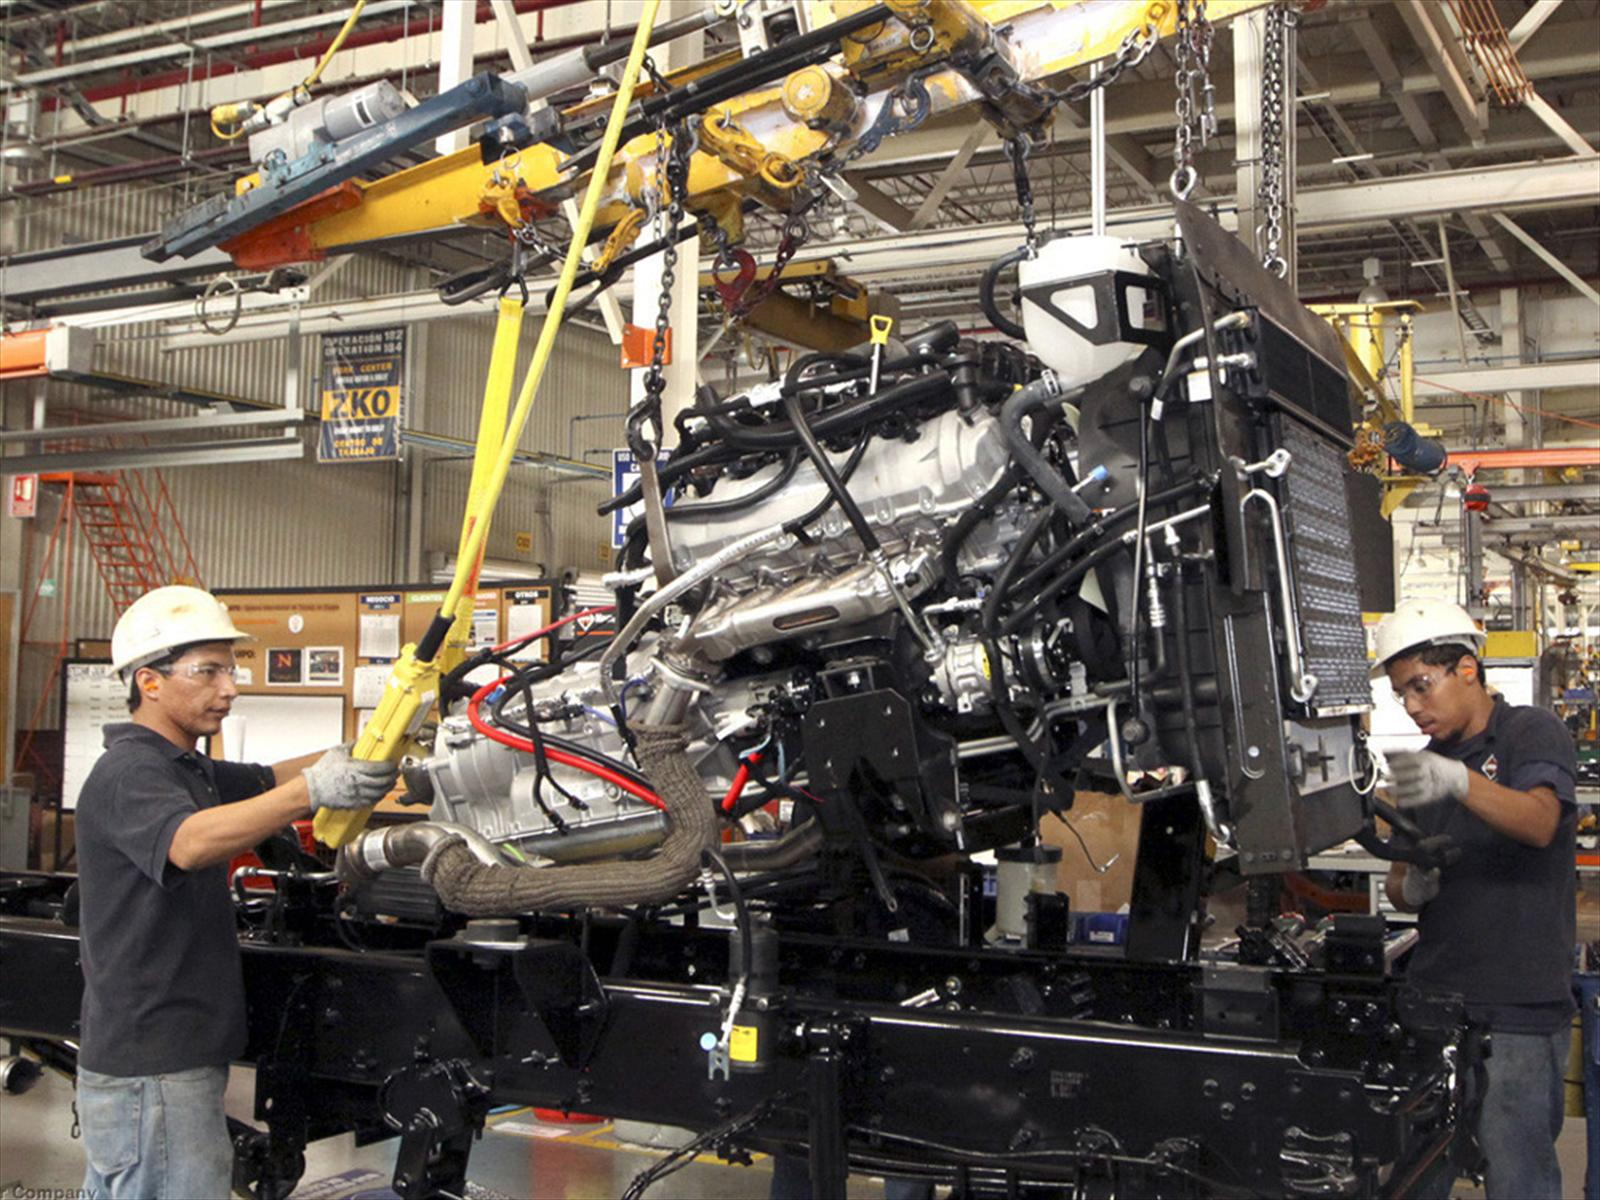
\includegraphics[width=\textwidth,height=0.8\textheight,keepaspectratio]{Ford in Mexico.jpg}
\end{frame}

\begin{frame} 
	\frametitle{\LARGE{Foreign Direct Investment}}
	Relevance of FDI to international politics: \pause 
	\begin{itemize}
		\item Enormous portion of world financial flows \pause 
		\item Unique regarding control of production \pause 
		\item Most directly related to actual economic activity \pause 
		\item Pertinent for economic growth \pause 
		\item Generates conflicts of interest
	\end{itemize}		
	
\end{frame}

\begin{frame} 
	\frametitle{\LARGE{Why Invest in Production Overseas?}}
	From the perspective of an MNC, why engage in FDI?
	\begin{itemize}
		\large{
			\item Direct advantages of new locations: \pause 
			\begin{itemize}
				\item Access to natural resources (e.g. ExxonMobil investing in Angola for oil). \pause 
				\item Selling to new markets and avoiding trade barriers (via horizontal FDI). \pause 
				\item Cheaper production costs, such as low-skilled labor (e.g. clothing produced in Bangladesh).  
			\end{itemize}
		}
	\end{itemize}
\end{frame}

\begin{frame} 
	\frametitle{\LARGE{Why Invest in Production Overseas?}}
	From the perspective of an MNC, why engage in FDI?
	\begin{itemize}
		\large{
			\item General advantages to operating internationally (regardless of specific locational advantages): \pause 
			\begin{itemize}
				\item Shifting profits between countries allows for tax avoidance. Ex: Google avoiding taxes on \$22 billion via a series of transfers so common they have a name: \href{https://www.investopedia.com/terms/d/double-irish-with-a-dutch-sandwich.asp}{Double Irish with a Dutch Sandwich.} \pause 
				\item Pre-investment bargaining advantages.\pause
				\item Cheaper supply chain input production.
			\end{itemize}
		}
	\end{itemize}
\end{frame}


% GSC image
\begin{frame}{\LARGE Global Supply Chains}
	\centering
	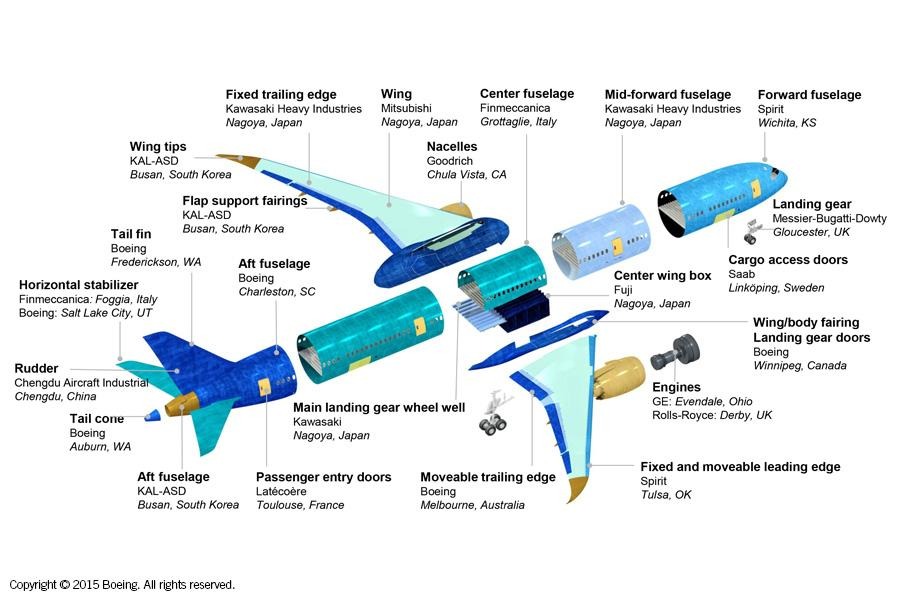
\includegraphics[width=\textwidth,height=0.8\textheight,keepaspectratio]{airplane gsc.jpg}
\end{frame}

\begin{frame} 
	\frametitle{\LARGE{Why Allow FDI?}}
	From the perspective of the state, what are the advantages?
	\begin{itemize}
		
		\item MNCs may have skills and technology that less-developed countries lack, especially in the case of natural resource extraction.  \pause 
		\begin{itemize}
			\item On-the-job training  \pause
			\item Technology transfer \pause 
		\end{itemize}
		\item Creates linkages in the host economy. \pause 
		\begin{itemize}
			\item E.g. a Coca-Cola production facility might spur the development of local bottle-making and bottling facilities, creating jobs. \pause 
		\end{itemize}
		\item Host governments can count on long-term, relatively stable tax revenues. \pause
		\item Creates relatively high-paying jobs for citizens in developing states.
		
	\end{itemize}
\end{frame}


% FDI by country 
\begin{frame}{\LARGE FDI by Country}
	\centering
	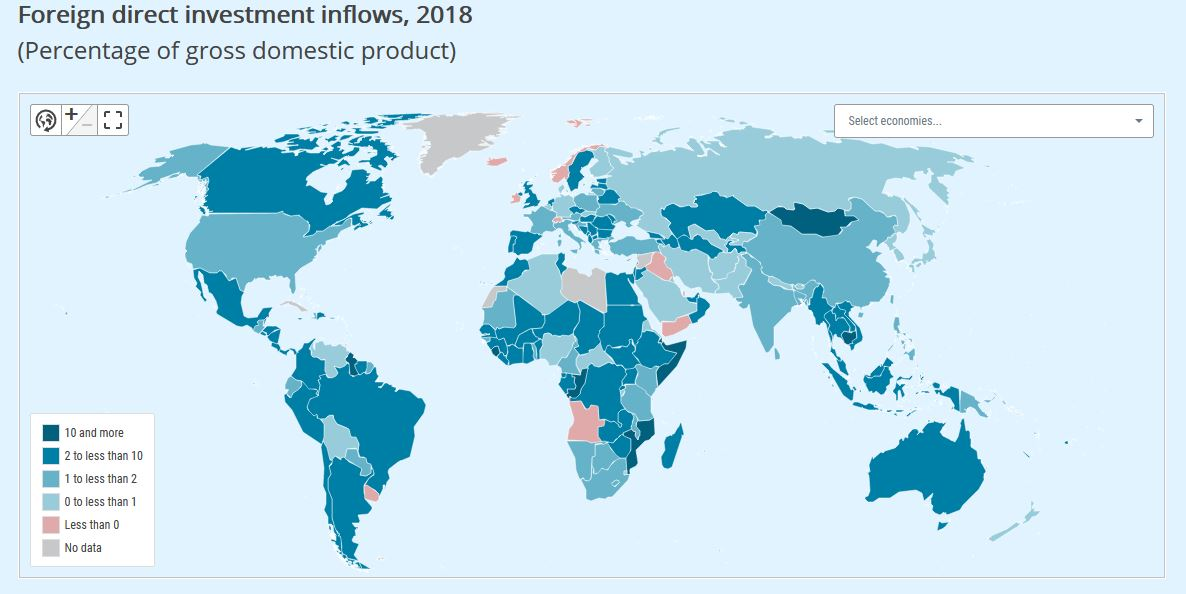
\includegraphics[width=\textwidth,height=0.8\textheight,keepaspectratio]{FDI by country.JPG}
\end{frame}

\begin{frame} 
	\frametitle{\LARGE{Why Prevent FDI?}}
	From the perspective of the state, what are the disadvantages?
	\begin{itemize}
		\large{
			\item FDI may drive local firms out of business. \pause 
			
			\item MNCs may work in enclaves, rather than integrating into local economies.   \pause
			\item Higher-paying positions may not materialize, or may be given to immigrating foreign workers. \pause 
			
			\item MNCs use \textbf{investor-state dispute settlement} provisions of bilateral investment treaties to undermine government labor or environmental regulations. \pause 
			
			\item Developing countries may lack capacity to monitor MNCs.  \pause 
			
			\item The MNC's home state may be upset that capital and production are moving elsewhere. 
		}
	\end{itemize}
\end{frame}



\begin{frame} 
	\frametitle{\LARGE{The Obsolescing Bargain}}
	In their interactions, an MNC and a host government face a particular kind of commitment problem called the \textbf{Obsolescing Bargain}:
	\begin{itemize}
		\item \textbf{Before they make their investment, MNCs have almost all the bargaining leverage.} \pause 
		\begin{itemize}
			\item They choose if and where to invest with no consequences for not investing in a given location. \pause 
			\item This may encourage a \textbf{race to the bottom} by developing countries to attract investments by cutting tax rates and labor safety laws, with negative impacts on worker safety \href{https://www.ilo.org/global/topics/geip/WCMS_614394/lang--en/index.htm}{(e.g. Rana Plaza Accident)}  
		\end{itemize}
	\end{itemize} 
\end{frame}

\begin{frame} 
	\frametitle{\LARGE{The Obsolescing Bargain}}
	In their interactions, an MNC and a host government face a particular kind of commitment problem called the \textbf{Obsolescing Bargain}:
	\begin{itemize}
		\item After the investment, an MNC has spent substantial time, money, and resources to establish their presence. \textbf{Now, due to the difficulty of easily exiting, host governments have all the leverage.} \pause 
		\begin{itemize}
			\item The government may \textbf{expropriate} income from the investment, either through nationalizing the investment or via stringent regulations and taxes. \pause
			\item Given the global shift toward FDI and free trade, MNCs are less concerned about nationalizations and more worried about \textbf{creeping expropriation} in which the state slowly increases its taxation, regulation, and ultimately control over the investment without nationalization.
		\end{itemize}
	\end{itemize}
	
\end{frame}



\begin{frame} 
	\frametitle{\LARGE{Conflict Between Hosts and MNCs}}
	\begin{itemize}
		\large{
			\item Hosts control taxation and regulation, up to the point of nationalizing or taking over the company, and host states have done so: \pause 
			\begin{itemize}
				\item Cuba famously nationalized US property (including casinos) after the 1959 revolution. \pause 
				\item Venezuela nationalized oil production in 1976. \pause
				\item More recently, Bolivia \href{https://www.cfr.org/backgrounder/bolivias-nationalization-oil-and-gas}{seized all oil and gas production facilities} in 2006.
			\end{itemize}
			\item Opposing interests between host state and MNC, as well as the shadow of the Obsolescing Bargain, can motivate economic conflict.
		}
	\end{itemize}
\end{frame}

\begin{frame} 
	\frametitle{\LARGE{Conflict Between Hosts and MNCs}}
	\begin{itemize}
		\large{
			\item MNCs have a number of possible options in such a conflict: \pause  
			\begin{itemize}
				\item Withholding capital and technology. \pause 
				\item Transferring profits out of the country. \pause 
				\item Withdrawing entirely, despite the costs of leaving. \pause 
				\item Lobbying the host governments (e.g. in Honduras prior to the Soccer War; concerns about dependency). \pause 
				\item Advocating for foreign, home government interference (e.g. United Fruit in Guatemala in 1954, ITT (\href{https://www.theguardian.com/business/1998/nov/08/observerbusiness.theobserver}{and Pepsi}) implicated in the 1973 Allende coup in Chile) 
			\end{itemize}
		}
	\end{itemize}
\end{frame}

\begin{frame} 
	\frametitle{\LARGE{Home Countries and MNCs}}
	\begin{itemize}
		\item The relationship between MNCs and their home/origin states has received far less attention from academics, until recently. \pause 
		\item Most post-industrial advanced economies have some kind of \href{https://www.jmfrri.gr.jp/english/430.html}{``reshoring"} initiative to bring back jobs lost to vertical FDI. \pause 
		\item These states have also tried to re-negotiate trade agreements to include more domestic jobs (e.g. provisions in the USMCA, a trade pact that replaced NAFTA). \pause 
		\item However, most reshoring jobs are linked with automated production, and thus aren't likely to address the needs from when jobs left.
	\end{itemize}
\end{frame}

\begin{frame} 
	\frametitle{\LARGE{What about Institutions?}}
	\begin{itemize}
		\item Thus far, global institutions have not been mentioned. Why? \pause 
		\item \textbf{There are no global international institutions that oversee FDI} in the same way that the IMF oversees flows of capital. But why not?
		\item First reason: no global public good is threatened if individual FDI ventures fail (unlike financial contagion). \pause 
		\item Second reason: Conflicts are only between individual countries and MNCs, decreasing the number of actors, making bargaining somewhat less complicated.  
		
	\end{itemize}
\end{frame}

\begin{frame} 
	\frametitle{\LARGE{What about Institutions?}}
	\begin{itemize}
		\item Third reason: states have some bargaining tactics that can force a compromise. \pause
		\begin{itemize}
			\item Governments can commit to avoid expropriation by tying their hands through tax cuts or regulatory commitments. \pause 
			\item Some states have bargaining advantage because of market size (China) or resource endowments (oil, gas, minerals, etc.).  
		\end{itemize}       
	\end{itemize}
\end{frame}

\begin{frame} 
	\frametitle{\LARGE{Bilateral Investment Treaties}}
	\begin{itemize}
		\item Instead of international institutions, countries use \textbf{bilateral investment treaties (BITs)} as smaller institutions to govern expectations regarding FDI between the two states. \pause 
		\begin{itemize}
			\item Which results in \href{https://investmentpolicy.unctad.org/international-investment-agreements/iia-mapping}{almost 2,600 active BITs as of this month.}
		\end{itemize}
		\item These contain \textbf{investor state dispute settlement} mechanisms: provisions for how to solve any dispute that occurs, often biased in favor of the MNC and its home state.	
	\end{itemize}
\end{frame}

%% FLS chart
\begin{frame}{\LARGE FDI Surge}
	\centering
	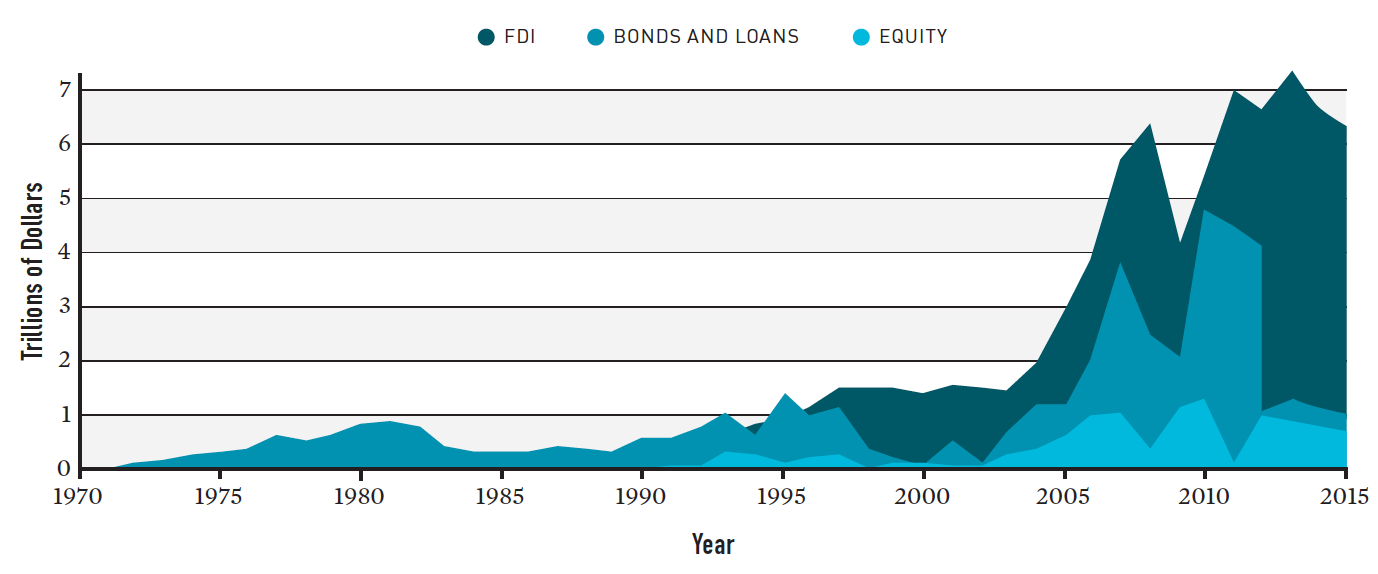
\includegraphics[width=\textwidth,height=0.8\textheight,keepaspectratio]{invest.png}
\end{frame}

\begin{frame} 
	\frametitle{\LARGE{Why the FDI Surge in LDCs?}}
	\begin{itemize}
		\large{
			\item Developing countries/less developed countries (LDCs), by definition, lack capital. \pause 
			\item Portfolio investments (bonds, stocks, loans) allow for local control of production, rather than MNC control. \pause 
			\begin{itemize}
				\item Crisis contagion means \textit{entire economy} may go out of control in a financial crisis. \pause  
				\item LDCs might struggle to control investment. \pause 
			\end{itemize}
			\item FDI, by contrast, cedes local control to MNCs. \pause 
			\begin{itemize}
				\item No connection to contagion, so creates more financial stability. \pause 
				\item Could generate more political instability?
			\end{itemize}
		}
	\end{itemize}
\end{frame}



%\begin{frame} 
%	\frametitle{\LARGE{Brooks, Cunha, Mosley (2015) Review}}
%	Group yourselves and answer the following:
%	\begin{itemize}
%		\item What is this article about? \pause 
		
%		\item What mechanism drives their argument? \pause 
		
%		\item What evidence do they provide? \pause 
		
%		\item How might this connect to other forms of investment (namely, FDI)? \pause 
		
%		\item What implications does this have for the rationalism framework? \pause 
%	\end{itemize}
%\end{frame}

\begin{frame} 
	\frametitle{\LARGE{Brooks, Cunha, Mosley (2015) Review}}
	\begin{itemize}
		\item What is this article about? \pause Investors evaluate a given state's sovereign debt through the use of heuristic groups of perceived peer states. 
		
		\item What mechanism drives their argument? \pause Heuristic grouping, in which investors sort states by perceived similarity rather than true risk.
		
		\item What evidence do they provide? \pause Quantitative.
		
		\item How might this connect to other forms of investment (namely, FDI)? \pause FDI decisions may be made in a similar way.
		
		\item What implications does this have for a rationalist framework? \pause Threatens its external validity.
	\end{itemize}
\end{frame}

\begin{frame} 
\frametitle{\LARGE{Summary}}
\begin{itemize}
	\item International finance can be divided into 3 categories: 
	\begin{itemize}
		\item Portfolio Investment
		\item Concessional Finance 
		\item Foreign Direct Investment
	\end{itemize} 
\end{itemize}
\end{frame}

\begin{frame} 
\frametitle{\LARGE{Summary: Portfolio Investment}}
\begin{itemize}
	\item Investors (lenders) seek out markets where their capital will return good interest rates, but balance this desire for returns with evaluations of market risk and political risk in their target countries.
	\item In the event of a financial crisis, a sector of the economy (and/or the government of a state) defaults on its debts. \pause
	\item This creates a strategic interaction between creditor and debtor, as debtors want all of their debt forgiven while creditors want to recover as much as they can. \pause
	\item This also leads to bargaining within the debtor state as creditors demand domestically unpopular austerity measures in return for restructuring the debt and providing new loans.
\end{itemize}
\end{frame}

\begin{frame} 
\frametitle{\LARGE{Summary: Portfolio Investment}}
\begin{itemize}
	\item The IMF tries to promote international financial stability, while also serving as a lender of last resort in financial crises. \pause
	\item The price of an IMF emergency loan is frequently harsh, unpopular austerity measures. \pause
	\item The IMF's decision-making process is dominated by the US and EU, leading to accusations that it is a tool of rich creditors despite its claims to impartiality.\pause
	\item This has fueled the rise of a potential alternative in the form of the AIIB. \pause
	\item In spite of the risks, international capital flows have continued to increase in recent decades.
\end{itemize}
\end{frame}

\begin{frame} 
	\frametitle{\LARGE{Summary: Concessional Finance}}
	\begin{itemize}
		\item Concessional finance describes giving or loaning money to the poorest developing states, which are considered too risky for traditional investors.
		\item Both rich states and international institutions do this, with the World Bank as the primary international institution providing concessional finance. \pause
		\item Generally deals in smaller amounts of capital than either portfolio investment or FDI. 	
	\end{itemize}
\end{frame}


\begin{frame} 
	\frametitle{\LARGE{Summary: FDI}}
	\begin{itemize}
		\large{
			\item MNCs are drivers of FDI, because of profit advantages to producing outside of their home state.  \pause 
			
			\item Host governments may welcome FDI because of its contributions to the economy. \pause 
			
			\item Both hosts and MNCs must overcome commitment problems in the form of the obsolescing bargain. \pause 
			
			\item MNCs and hosts can clash over the distribution of benefits from the investment. \pause 
			
			\item FDI is still generally attractive to LDCs because of its relative stability, though it may create political conflict.
		}
	\end{itemize}
\end{frame}

\begin{frame} 
\frametitle{\LARGE{To Ponder...}}
    \centering
    \Large{Given the risks of international finance and the increasing openness of the world to it, what are the distributional consequences at the state level? At the firm level? In domestic politics? }
\end{frame}




\end{document}
